\documentclass[aspectratio=169]{beamer}
%\documentclass{beamer}

%%%%%%%%%%%%%%%%%%%%%%%%%%%%%%%%%%%%%%%%%%%%%%%%%%%%%%%%%%%%%%%%%%%%%%%%%%%%%%%%
%%%
%%% packages
%%%

%%%
%%% encoding and language set
%%%

%%% ngerman: language set to new-german
\usepackage[english]{babel}

%%% babel: language set (can cause some conflicts with package ngerman)
%%%        use it only for multi-language documents or non-german ones
%\usepackage[ngerman]{babel}

%%% inputenc: coding of german special characters
\usepackage[utf8]{inputenc}

%%% fontenc, ae, aecompl: coding of characters in PDF documents
\usepackage[T1]{fontenc}
\usepackage{ae,aecompl}

%%%
%%% technical packages
%%%

%%% amsmath, amssymb, amstext: support for mathematics ttt
%\usepackage{amsmath,amssymb,amstext}

%%% psfrag: replace PostScript fonts
\usepackage{psfrag}

%%% listings: include programming code
\usepackage{listings}
\usepackage{courier}
\lstset{basicstyle=\footnotesize\ttfamily,breaklines=true}

%%% units: technical units
\usepackage{units}

%%% tiefgestellte zahlen
\usepackage{subscript}


\usepackage[official]{eurosym}

\usetheme{metropolis}           % Use metropolis theme

\usepackage{xspace}




%%%%%%%%%%%%%%%%%%%%%%%%%%%%%%%%%%%%%%%%%%%%%%%%%%%%%%%%%%%%%%%%%%%%%%%
%%% Title stuff

\title{Angel Introduction: Camera and Video Mixer}
%\date{\today \currenttime}
\author{frederik, sophie, jwacalex, eric, pat}
\institute{C3VOC}

%%%%%%%%%%%%%%%%%%%%%%%%%%%%%%%%%%%%%%%%%%%%%%%%%%%%%%%%%%%%%%%%%%%%%%%%%%%%%%%%
%%%
%%% begin document
%%%

\begin{document}

%\pagenumbering{roman} %% small roman page numbers

%%% include the title
% \thispagestyle{empty}  %% no header/footer (only) on this page
\maketitle

%%% start a new page and display the table of contents
\begin{frame}{Inhalt}
\tableofcontents
\end{frame}
%%% start a new page and display the list of figures
% \newpage
% \listoffigures

%%% start a new page and display the list of tables
% \newpage
% \listoftables

%%% display the main document on a new page 
\newpage

% \pagenumbering{arabic} %% normal page numbers (include it, if roman was used above)

%%%%%%%%%%%%%%%%%%%%%%%%%%%%%%%%%%%%%%%%%%%%%%%%%%%%%%%%%%%%%%%%%%%%%%%%%%%%%%%%
%%%
%%% begin main document

%notes
%%%%%%%%%%%%%%%%%%%%%%%%%%%%%

%%%%%%%%%%%%%%%%%%%%%%%%%%%%%%%%%%%%%%%%%%%%%%%%%%%%%%%%%%%%%%%%%%%%%%
%%% Slides

\section{General Info}
\begin{frame}{General Info I}
	\begin{itemize}
		\item All talks get recorded and archived forever
		\item Consistent quality
		\item No postproduction of individual signals.
		\item Livestream content is the same as the one recorded and published
		\item Less mistakes $\Rightarrow$ better recodings.
		\item Stream observer shifts
	\end{itemize}
\end{frame}


\begin{frame}{General Info II}
	\begin{itemize}
		\item Introduction Meeting here
		\item Complete overview for all new angels
		\item Short diff for experienced ones
		\item Shift distribution every day 17:00 - 18:00 in CCL room 11.
		\item Feedback loop and review at those meetings
		\item Slides available online: \texttt{https://github.com/voc/engelschulung}
	\end{itemize}
	\begin{figure} 
		\centering
		
\includegraphics[height=0.4\textheight]{images/qr-code.png}
	\end{figure}
\end{frame}

\section{Angeltypes}
\begin{frame}{Angeltypes}
	\begin{itemize}
		\item Camera Angels
		\item Video Mixer Angels
		\item Stream Observing Angels
		\item A/V Technician
		\item Stage Manager
	\end{itemize}
\end{frame}

\begin{frame}{Camera Angels}
	\begin{itemize}
		\item Operate the fixed cameras in the lecture halls. 
		\item Usually, two camera angels per lecture hall 
		\item Camera angels will communicate with the Video-Mixer-Angel via intercom,
		\item Get instructions to shoot in certain ways. 
		\item Maintain good camera settings.
		\item Can sign up for the shifts in the Engelsystem themselves.
	\end{itemize}
\end{frame}

\begin{frame}{Video Mixer Angels}
	\begin{itemize}
		\item Switch the video feed between different sources. 
		\item Mixed video feed is used for both the live-stream and the recordings 
		\item You decide which picture, respectively source, is most interesting/important at each moment.
		\item Work proactively with camera angels through the intercom, 
		\item Challenging talks, with assistance from an external "image composition director" joining the intercom channel.
	\end{itemize}
\end{frame}

\begin{frame}{Stream Observing Angels}
	\begin{itemize}
		\item Open for all camera and mixing angels
		\item Reflecting the work of colleagues from an audience perspective.
		\item Examine streams for issues 
		\item Keep track of sequences appearing hard to consume or violating our rule set. 
		\item Positive and negative remarks 
		\item Constructive feedback 
		\item Instantly report severe issues like "there is no signal" to the VOC Helpdesk.%%TODO Eskalationsstufen
		\item Self evaluation and not meant as external monitoring. 
	\end{itemize}
\end{frame}

\begin{frame}{A/V Technician}
	\begin{itemize}
		\item 2nd level support in the lecture halls. 
		\item Responsible for camera and mixer angels
		\item Familiar with the equipment that is used. 
		\item Able to fix (nearly) all the issues. 
		\item is on intercom %%TODO We have a partyline, are the AV techs really on the intercom?
	\end{itemize}
\end{frame}


\begin{frame}{Stage Manager}
\begin{itemize}
	\item is responsible for the lecture hall, especially
	\begin{itemize}
		\item crowd control
		\item time keeping
		\item last minute issues 
	\end{itemize}
	\item carries the radio for emergency communication
	\item Talks to the A/V technician so usually they don't  interact with camera and mixer angels.
\end{itemize}
\end{frame}

\begin{frame}{A/V Technician \& Stage Manager}
\begin{itemize}
	\item have the same shift slots (4h) together
	\item Camera and mixer angels: The A/V technician is responsible for you, not the stage manager.
	\item Stage Manager is communication gateway to heralds.
\end{itemize}
\end{frame}



\section{Camera Hardware}
\begin{frame}{Hardware Camera Controls Panasonic}
	\begin{columns}[T,onlytextwidth]
		\column{0.5\textwidth}
	\begin{figure} 
		\centering
		\includegraphics[width=0.9\textwidth]{images/panasonic_seitenansicht_objektiv.png}
		\caption{Panasonic Cam}
	\end{figure}
		\column{0.5\textwidth}
		Cameras are in manual mode because of difficult lighting situation.
		\begin{description}
			\item[Left Ring/red] Focus - control sharpness of the image.
			\item[Middle Ring/green] Zoom - vary the focal length.
			\item[Right Ring/blue] Iris - don't touch if you don't know why you should. For lighting issues talk to the A/V tech via intercom.%%can we train for Iris?
		\end{description}
	\end{columns}
\end{frame}

\begin{frame}{Hardware Camera Controls JVC}
	\begin{columns}[T,onlytextwidth]
		\column{0.5\textwidth}
	\begin{figure} 
		\centering
		\includegraphics[width=0.9\textwidth]{images/jvc_seitenansicht_objektiv.png}
		\caption{JVC Cam}
	\end{figure}
		\column{0.5\textwidth}
		Cameras are in manual mode because of difficult lighting situation.
		\begin{description}
			\item[Left Ring/red] Focus - control sharpness of the image.
			\item[Middle Ring/green] Zoom - vary the focal length.
%			\item[Right Ring/blue] Iris - don't touch if you don't know why you should. For lighting issues talk to the A/V tech via intercom.
		\end{description}
	\end{columns}
\end{frame}

\begin{frame}{Zoom Control Panasonic}
	\begin{columns}[T,onlytextwidth]
		\column{0.5\textwidth}
	\begin{figure} 
		\centering
		\includegraphics[width=0.99\textwidth]{images/panasonic_zoom.png}
		\caption{Panasonic Cam}
	\end{figure}
		\column{0.5\textwidth}
		\begin{itemize}
			\item For smooth zoom use the zoom buttons.
			\item Gentle touch $\Rightarrow$ slow zoom
			\item Top Buttons fixed speed
		\end{itemize}
	\end{columns}
\end{frame}

\begin{frame}{Zoom Control JVC}
	\begin{columns}[T,onlytextwidth]
		\column{0.5\textwidth}
	\begin{figure} 
		\centering
		\includegraphics[width=0.9\textwidth]{images/jvc_zoom.png}
		\caption{JVC Cam}
	\end{figure}
		\column{0.5\textwidth}
		\begin{itemize}
			\item For smooth zoom use the zoom buttons.
			\item Gentle touch $\Rightarrow$ slow zoom
			\item Top Buttons fixed speed
		\end{itemize}
	\end{columns}
\end{frame}


\begin{frame}{Display Indicators Panasonic}
	\begin{columns}[T,onlytextwidth]
		\column{0.5\textwidth}
	\begin{figure} 
		\centering
		\includegraphics[width=0.9\textwidth]{images/panasonic_display_description.png}
		\caption{Panasonic Display Indicators}
	\end{figure}
		\column{0.5\textwidth}
		\begin{description}
			\item[Rec Indicator] The recording must always run, even during the break.
			\item[Focal Indicator] Use only manual focus!
			\item[Remaining Time] It must have enough remaing time before talk.
		\end{description}
		\metroset{block=fill}
		\begin{alertblock}{Alert}
			Alert the A/V-Technician if something's wrong.
		\end{alertblock}
	\end{columns}
\end{frame}

\begin{frame}{Display Indicators JVC}
	\begin{columns}[T,onlytextwidth]
		\column{0.5\textwidth}
	\begin{figure} 
		\centering
		\includegraphics[width=0.9\textwidth]{images/jvc_display_description.png}
		\caption{Panasonic Display Indicators}
	\end{figure}
		\column{0.5\textwidth}
		\begin{description}
			\item[Rec Indicator] The recording must always run, even during the break.
			\item[Focal Indicator] Use only manual focus!
		\end{description}
		\metroset{block=fill}
		\begin{alertblock}{Alert}
			Alert the A/V-Technician if something's wrong.
		\end{alertblock}
	\end{columns}
\end{frame}


\begin{frame}{Tripod Handle Controls}
	\begin{columns}[T,onlytextwidth]
	\column{0.5\textwidth}
	\begin{figure} 
		\centering
		\includegraphics[width=0.7\textwidth]{images/tripod-handle.jpeg}
		\caption{Tripod Handle}
	\end{figure}

	\column{0.5\textwidth}
	Beware: various models in use.
	\begin{description}
		\item[Zoom Control] lever above red ring
		\item[Red Button] Start/stop recording, don't touch
		\item[Other Buttons] markings on the handle
    \end{description}
	\end{columns}
\end{frame}

\begin{frame}{Tripod}
	\begin{columns}[T,onlytextwidth]
	\column{0.4\textwidth}
	\begin{figure} 
		\centering
		\includegraphics[width=0.9\textwidth]{images/tripod-complete.png}
		\caption{Tripod}
	\end{figure}
	
	\column{0.6\textwidth}
	\begin{itemize}
			\item Should be level - check the water bubble.
			\item Variable brakes - can be adjusted to your needs.
			\item Tilt axis should be balanced, so that the camera doesn't tilt up or down on its own.
			\item Pan axis is needed all of the time. Set it so you can do smooth pans all over the stage.
		\end{itemize}
		\metroset{block=fill}
		\begin{alertblock}{Alert}
			Alert the A/V-Technician if something's wrong or misplaced.
		\end{alertblock}
	\end{columns}
\end{frame}

\begin{frame}{SD-Card Recording}
		\begin{itemize}
			\item Two SD-Cards in every Camera
			\item Backup Recording
			\item Turn on Recording before first shift in the morning -> Red Dot somewhere in the Display.
			\item Control Recording Time remaining. 
		\end{itemize}
		\metroset{block=fill}
		\begin{alertblock}{Alert}
			Alert the A/V-Technichian if something's wrong or not running.
		\end{alertblock}
\end{frame}

\section{Camera Positions and Angles}
\begin{frame}{Map of the fair grounds}
	\begin{figure} 
		\centering
		\includegraphics[height=0.9\textheight]{images/planmessegelaende_rotelinien.png}
	\end{figure}
\end{frame}

\begin{frame}{Rooms in CCL}
	\begin{figure} 
		\centering
		\includegraphics[height=0.9\textheight]{images/congress_center_leipzig_querschnitt.jpg}
	\end{figure}
\end{frame}

\begin{frame}{Saal Borg}
	\begin{figure} 
		\centering
		\includegraphics[height=0.9\textheight]{images/SaalB.png}
	\end{figure}
\end{frame}

\begin{frame}{Camera 1 - Closeup Camera}
		\begin{block}{Content}
			\begin{itemize}
				\item The Speaker is your best friend
				\item Keep them always in frame
				\item Default for all composition modes
			\end{itemize}
		\end{block}
		
		\begin{block}{Framing}
			\begin{itemize}
				\item The upper part of their body + head + a bit of headroom.
				\item Stay close to his/her eyeline on the upper third line.
			\end{itemize}
		\end{block}

		\begin{alertblock}{Alerts}
			\begin{itemize}
				\item Anticipate movement, stay alert
				\item Leave some room where they want to move next.
			\end{itemize}
		\end{alertblock}
\end{frame}

\begin{frame}{Camera 1 - Closeup Camera}
	Example Shots I
	\begin{figure} 
		\centering
		\includegraphics[width=0.7\textwidth]{images/closeup1.jpg}
		\caption{Good Closeup Shot}
	\end{figure}
\end{frame}

\begin{frame}{Camera 1 - Closeup Camera}
	Example Shots II
	\begin{figure} 
		\centering
		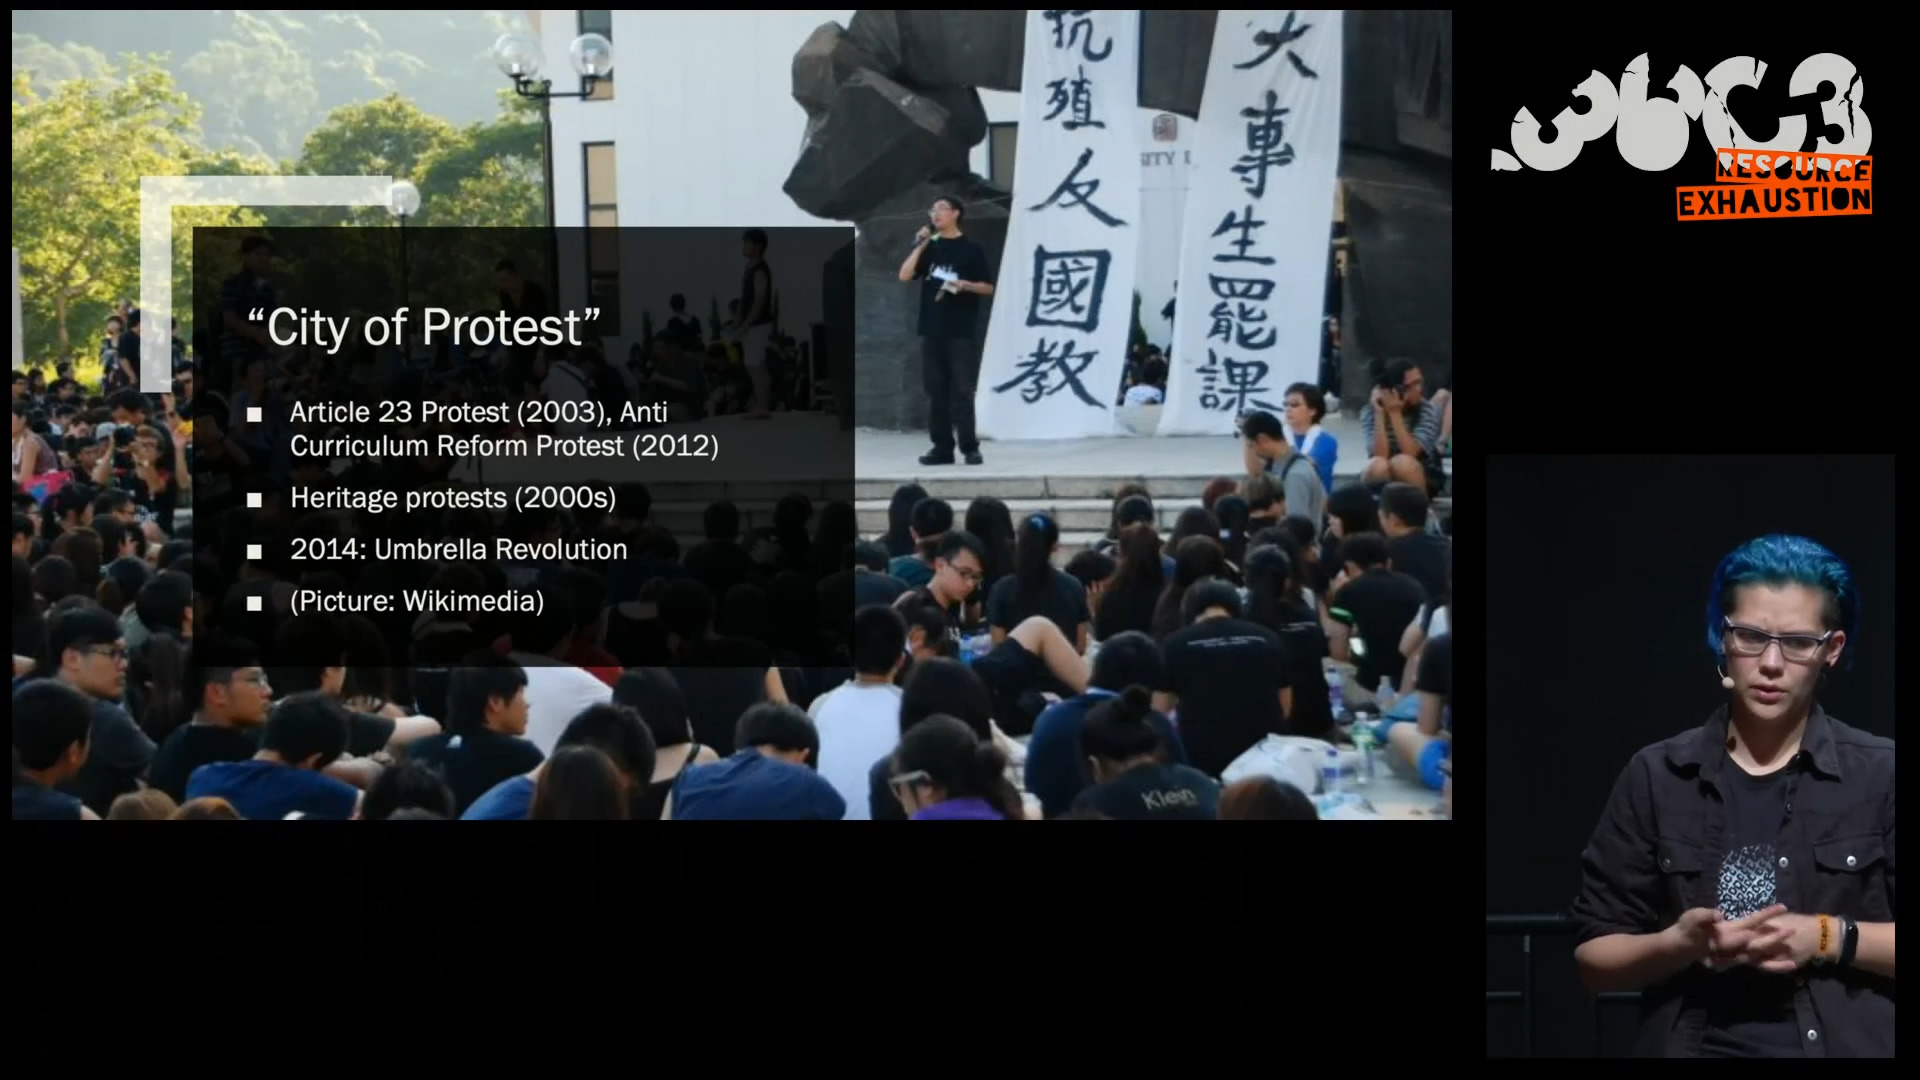
\includegraphics[width=0.7\textwidth]{images/closeup2.jpg}
		\caption{Good Closeup in Supersource}
	\end{figure}
\end{frame}

\begin{frame}{Camera 1 - Closeup Camera}
	Bad Shots I
	\begin{figure} 
		\centering
		\includegraphics[width=0.7\textwidth]{images/closeup-bad1.png}
		\caption{Half a head - not good.}
	\end{figure}
\end{frame}

\begin{frame}{Camera 1 - Closeup Camera}
	Bad Shots II
	\begin{figure} 
		\centering
		\includegraphics[width=0.7\textwidth]{images/closeup-bad2.png}
		\caption{Too Far out for a good supersource image.}
	\end{figure}
\end{frame}


\begin{frame}{Camera 2 - Medium Camera}
		\begin{block}{Content}
			\begin{itemize}
				\item Context around the speaker
				\item If there are two or more speakers choose the other one
			\end{itemize}
		\end{block}
		
		\begin{block}{Framing}
			\begin{itemize}
				\item Speaker from Head to Toes
				\item Stay close to his/her eyeline on the upper third line.
			\end{itemize}
		\end{block}

		\begin{alertblock}{Alerts}
			\begin{itemize}
				\item Anticipate movement.
				\item Leave some room where they want to move next.
				\item Fallback Camera if the Closeup Camera can't keep up.
			\end{itemize}
		\end{alertblock}
\end{frame}

\begin{frame}{Camera 2 - Medium Camera}
	\textbf{Good Shots I}
	\begin{figure} 
		\centering
		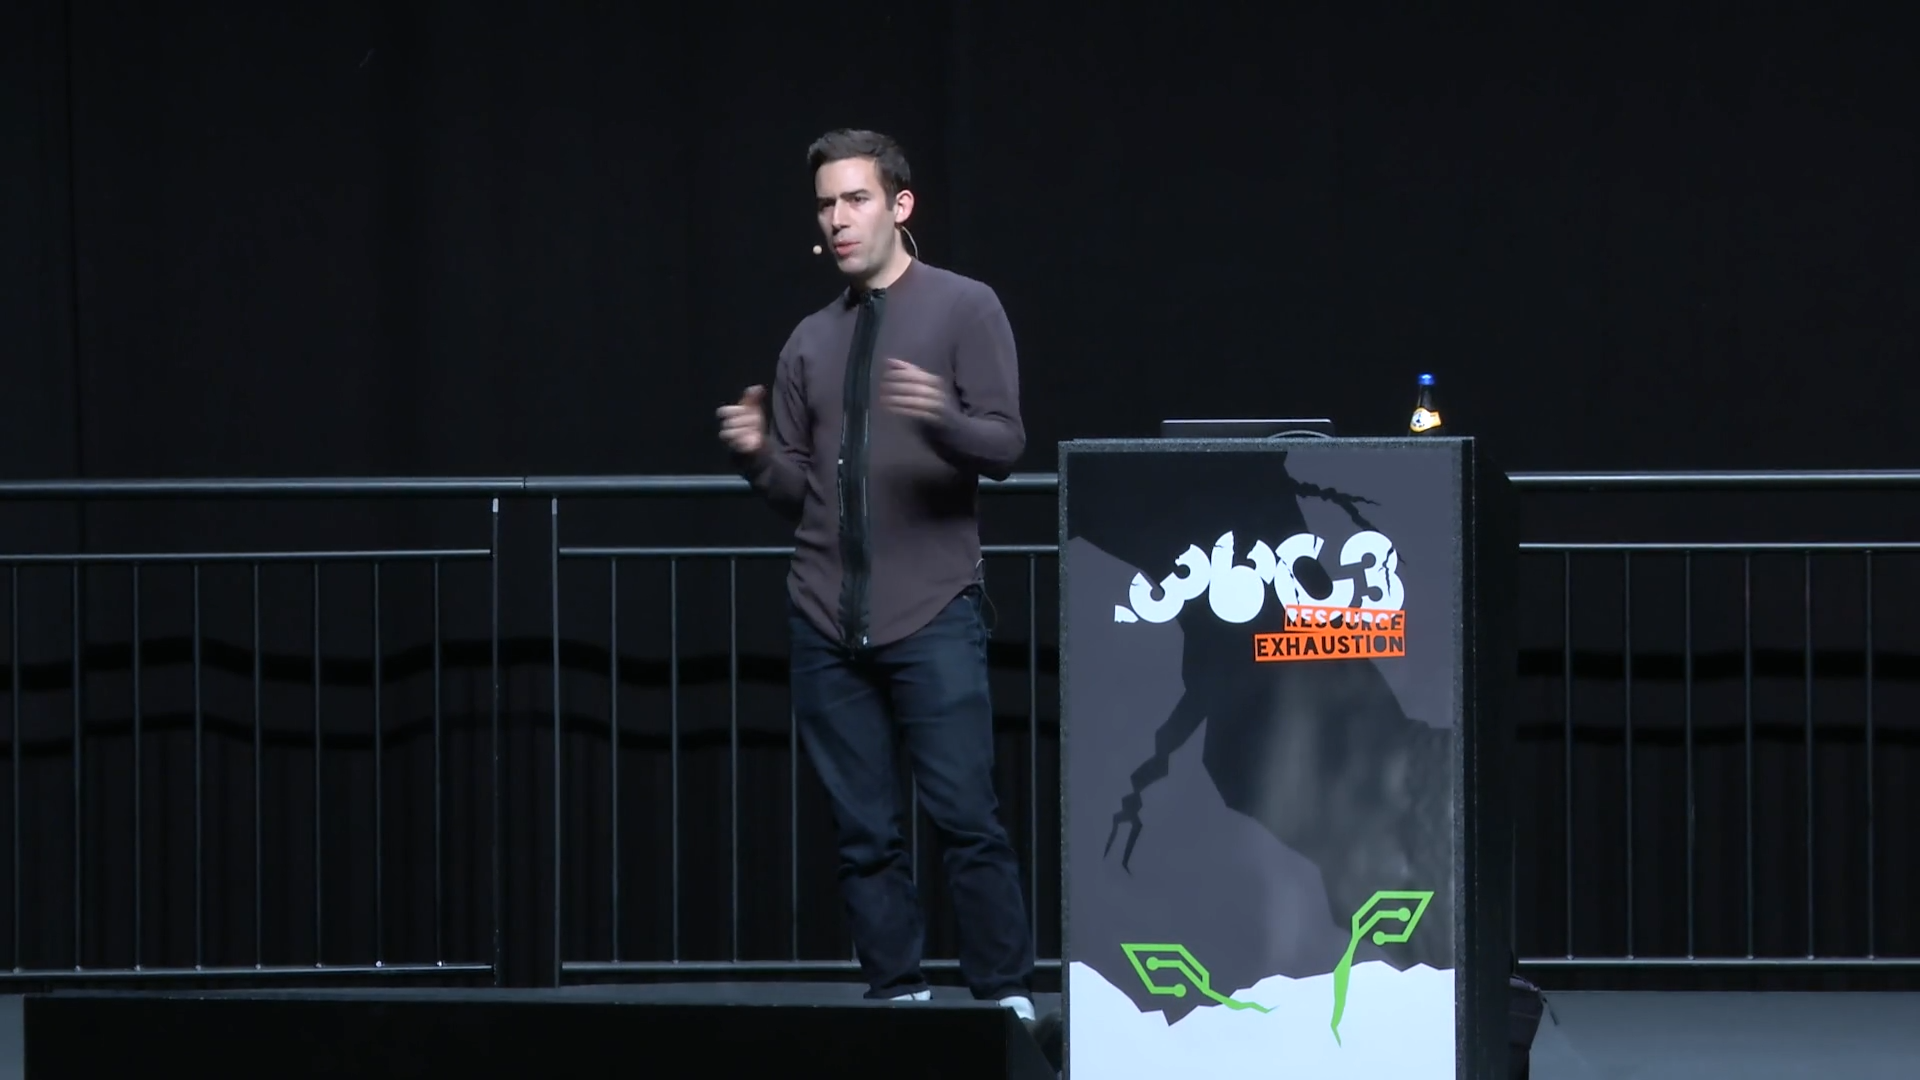
\includegraphics[width=0.7\textwidth]{images/medium1.png}
		\caption{Good Context image.}
	\end{figure}
\end{frame}

\begin{frame}{Camera 2 - Medium Camera}
	\textbf{Good Shots II}
	\begin{figure} 
		\centering
		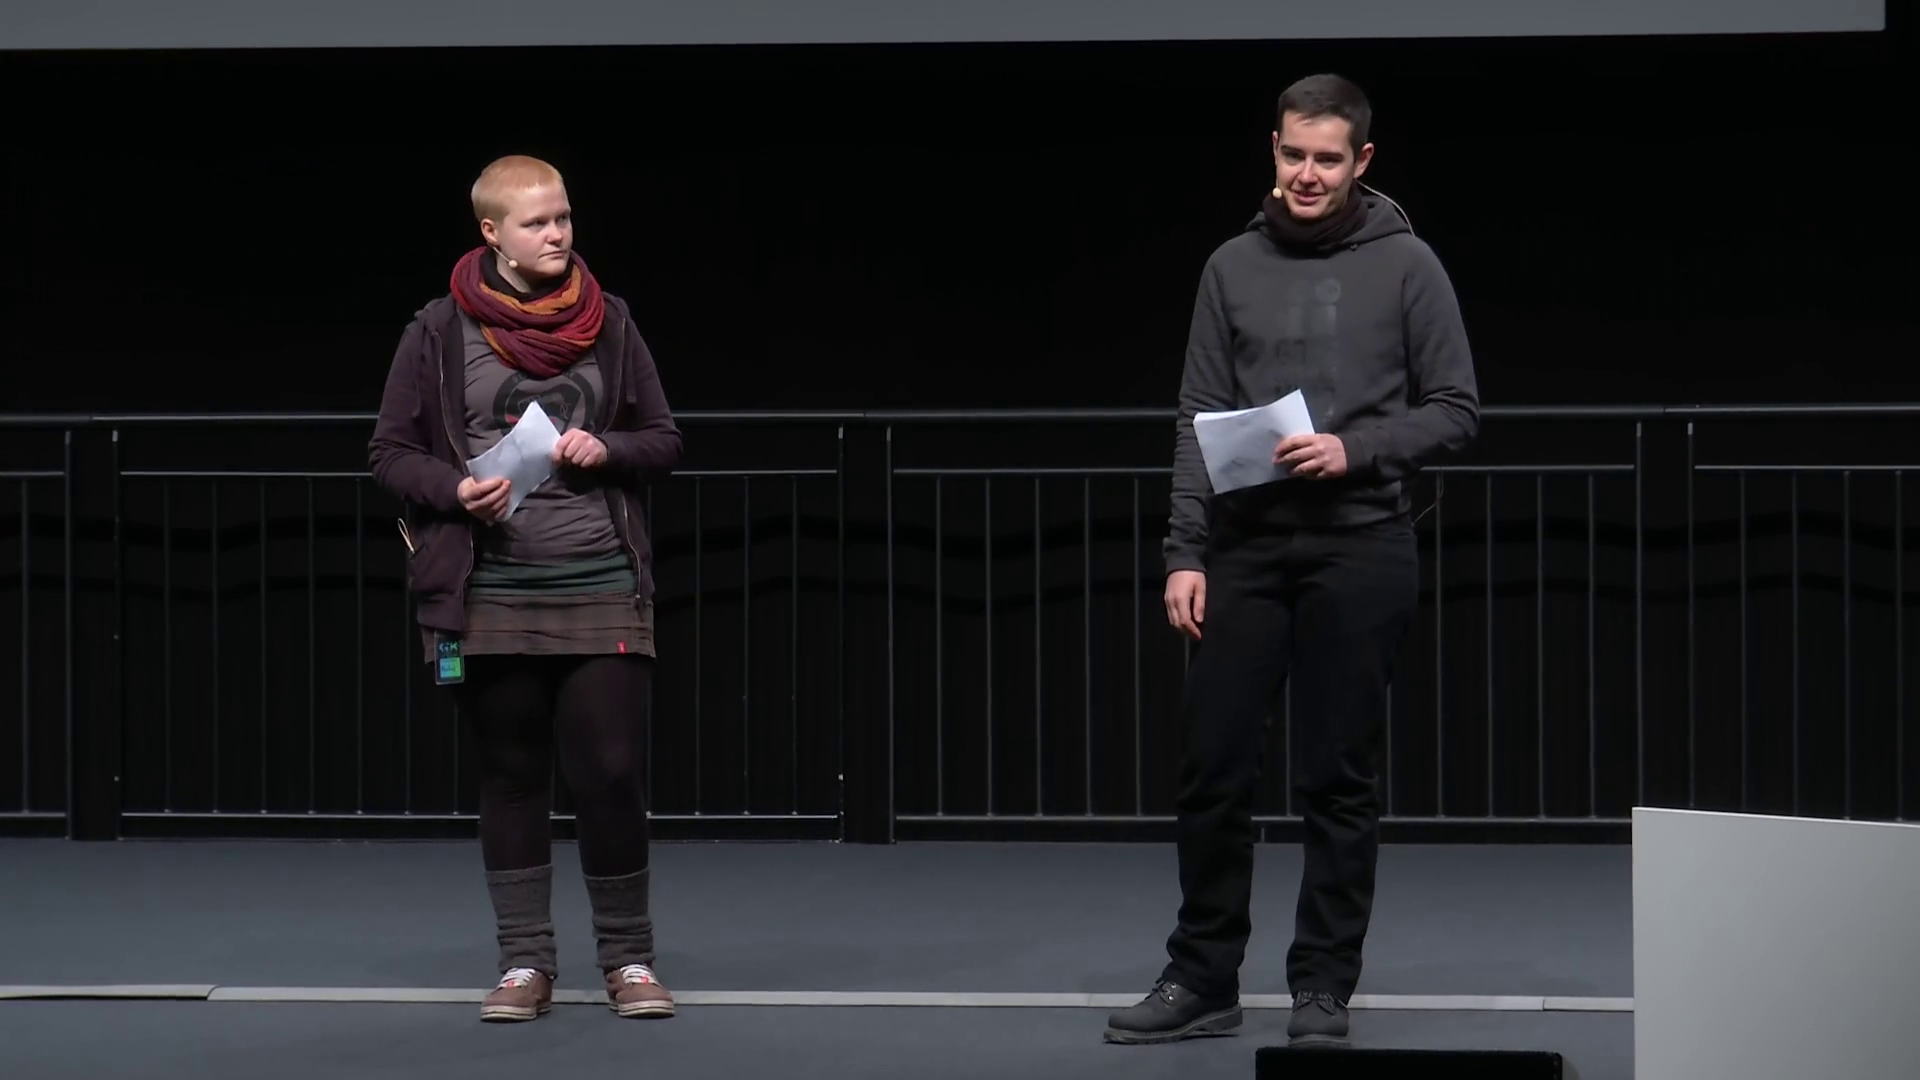
\includegraphics[width=0.7\textwidth]{images/Speaker_full.png}
		\caption{Two Speakers.}
	\end{figure}
\end{frame}

\begin{frame}{Camera 3 - Wide Shot}
		\begin{block}{Framing}
			\begin{itemize}
				\item Covers the whole stage.
				\item A bit of small audience for context.
				\item Statically set.
			\end{itemize}
		\end{block}

		\begin{alertblock}{Alerts}
			\begin{itemize}
				\item Needs no attention. 
				\item Fallback Camera if all else fails 
				\item Beautifully captures standing ovations
			\end{itemize}
		\end{alertblock}
\end{frame}

\begin{frame}{Camera 3 - Wide Shot}
	\begin{figure} 
		\centering
		\includegraphics[width=0.7\textwidth]{images/wide-shot.jpeg}
	\end{figure}
\end{frame}

\section{Intercom} %%Neue Fotos vom Intercom
 \begin{frame}{Intercom}
 	\begin{figure} 
 		\centering
 		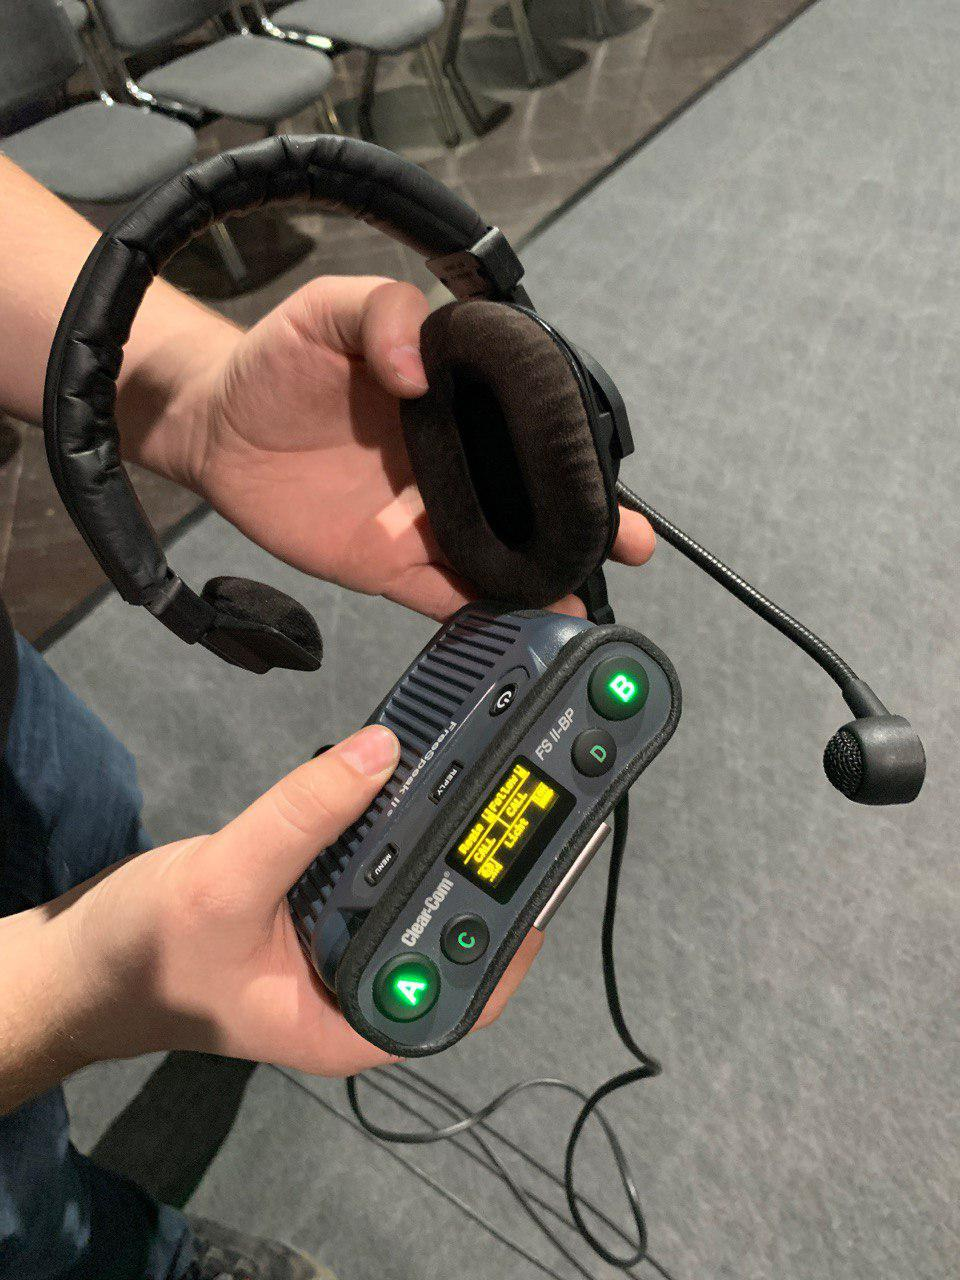
\includegraphics[width=0.4\textwidth]{images/intercom_36c3.jpg}
 	\end{figure}
	%\begin{columns}[T,onlytextwidth]
	%\column{0.5\textwidth}
	%	\begin{figure} 
	%	\centering
	%	\def\svgwidth{1\textwidth}
	%	\includegraphics[width=0.9\textwidth]{images/intercom.png} 
	%	\end{figure}
	%\column{0.5\textwidth}
	%\begin{figure} 
	%	\centering
	%	\def\svgwidth{1\textwidth}
	%	\includegraphics[width=0.93\textwidth]{images/bolero.jpg} 
	%\end{figure}
	%\end{columns}
\end{frame}

\section{Video Mixer Tools}

\begin{frame}{Voctomix}
	\begin{columns}[T,onlytextwidth]
	\column{0.5\textwidth}
	\begin{figure} 
		\centering
		\includegraphics[width=1\textwidth]{images/voctomix.png}
		\caption{Voctogui}
		\label{fig:voctogui1}
	\end{figure}

	\column{0.5\textwidth}
	\begin{description}
		\item[Previews] Small images on the left 
		\item[Program] Large, middle, what everyone on the internet sees.
		\item[Composition] Top row.
		\item[Blue] Select A
		\item[Red] Select B
		\item[Stream Blank] For breaks when nothing should be streamed.
     \end{description}
	\end{columns}
\end{frame}

\begin{frame}{Software Video Mixer - Voctogui}
	\begin{figure} 
		\centering
		\includegraphics[width=.9\textwidth]{images/voctomix.png}
		\caption{Voctogui}
	\end{figure}
\end{frame}

\begin{frame}{Voctomix2}%%TODO finish slide
	\begin{itemize}
		\item Voctomix2 Setup in hall D and Chaos West Stage
		\item New GUI and features
		\item We'd like to have your feedback --> There are signs with a link to a feedback pad at both stages 
	\end{itemize}
\end{frame}

\begin{frame}{Software Video Mixer - Voctomix2}%%TODO Voctomix2
	\begin{figure} 
		\centering
		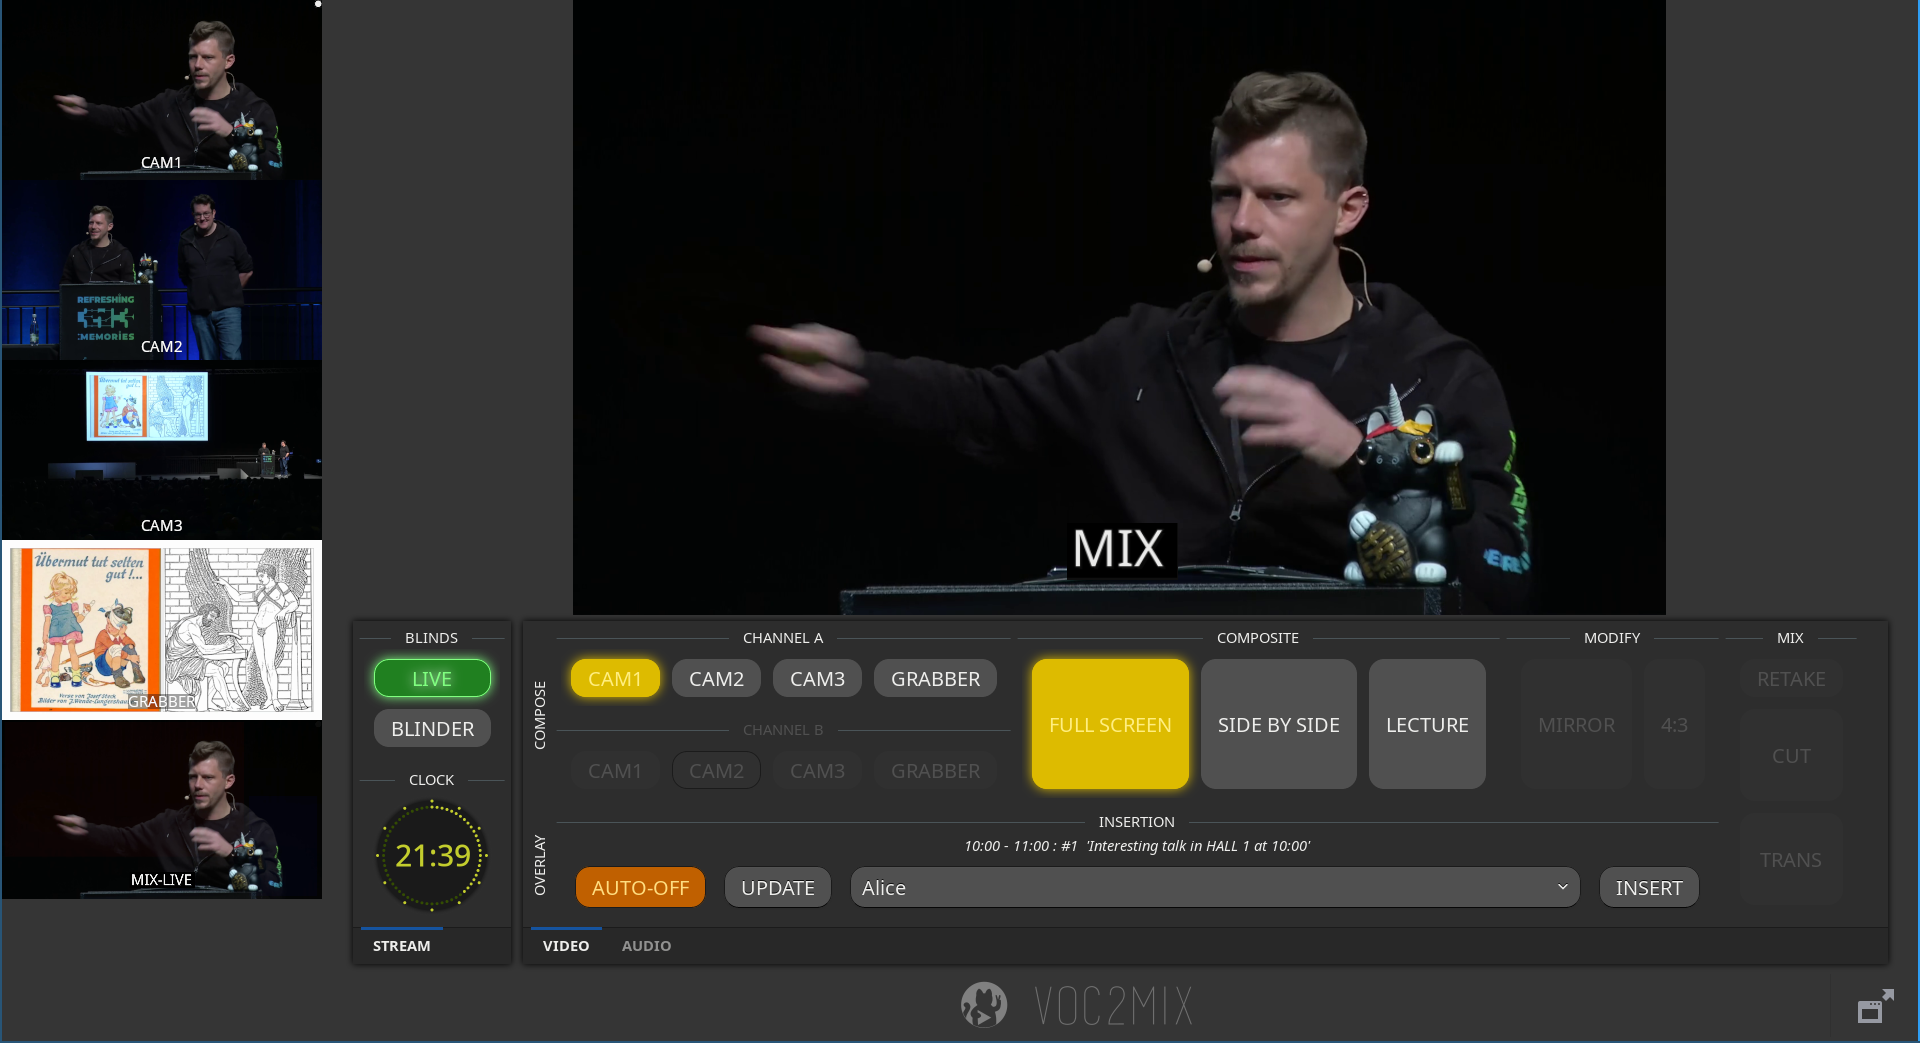
\includegraphics[width=.9\textwidth]{images/voctomix2_1.png}%%TODO Add Voctomix2 image
		\caption{Voctomix2}
	\end{figure}
\end{frame}

\begin{frame}{Software Video Mixer - Voctomix2}%%TODO Voctomix2
	\begin{figure} 
		\centering
		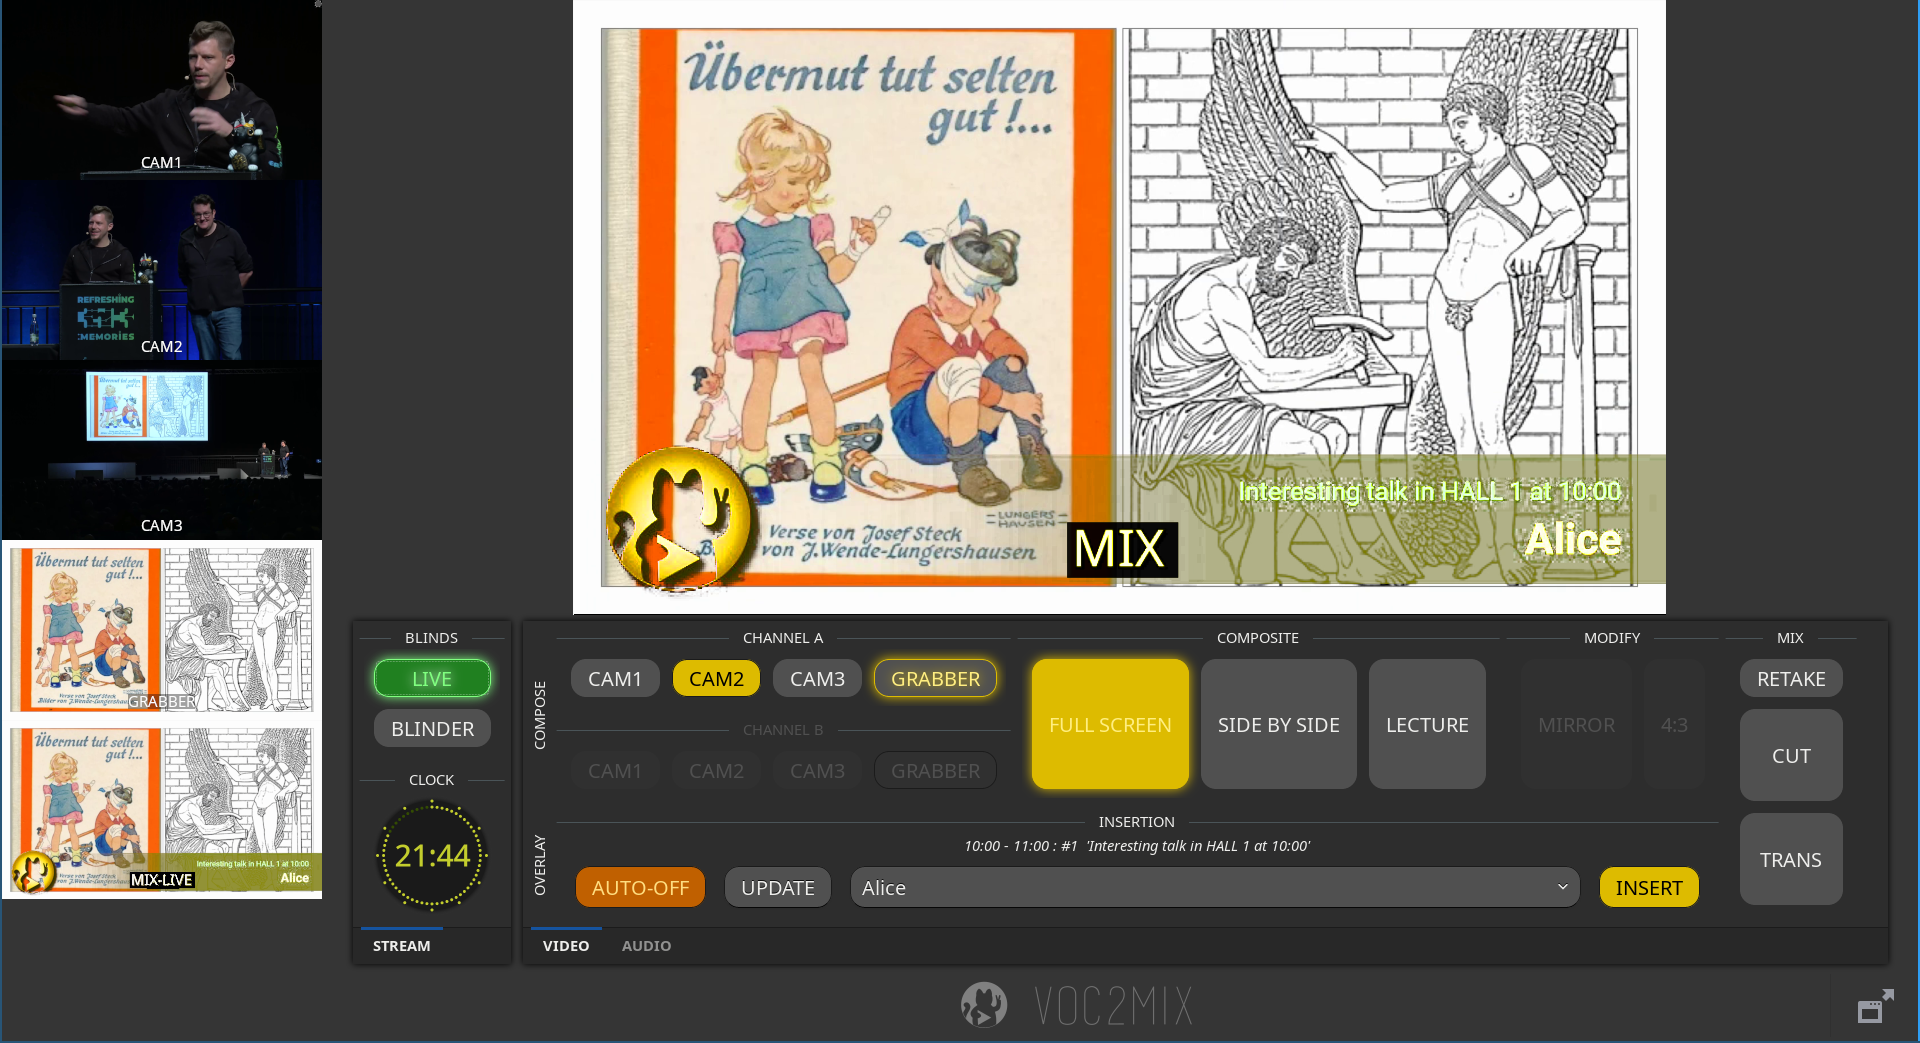
\includegraphics[width=.9\textwidth]{images/voctomix2_2.png}%%TODO Add Voctomix2 image
		\caption{Voctomix2}
	\end{figure}
\end{frame}

\begin{frame}{Software Video Mixer - Voctomix2}%%TODO Voctomix2
	\begin{figure} 
		\centering
		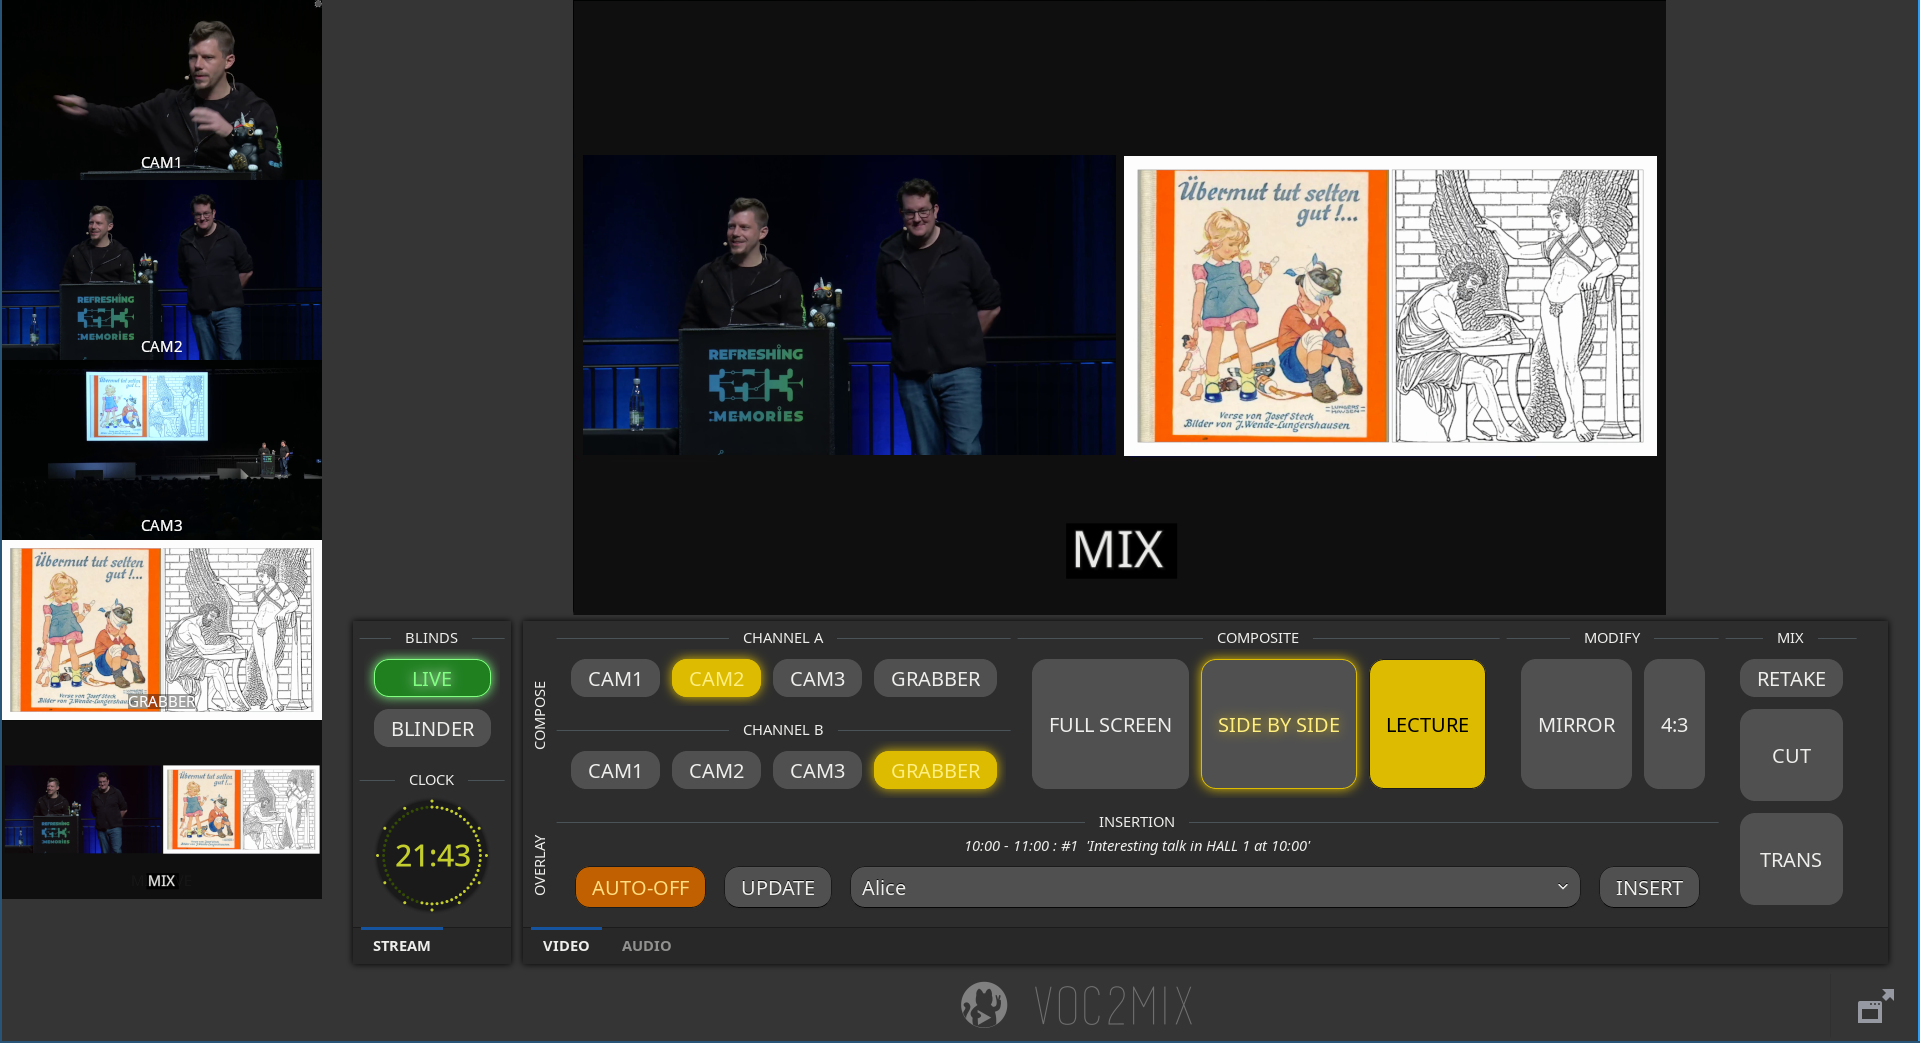
\includegraphics[width=.9\textwidth]{images/voctomix2_3.png}%%TODO Add Voctomix2 image
		\caption{Voctomix2}
	\end{figure}
\end{frame}




\section{Video Mixing Guidelines}
\begin{frame}{Mixing Guidelines - Hard Rules}
	\begin{itemize}
		\item \textbf{All} you are doing is \textbf{recorded} and will be published. \alert{\textbf{Don't make mistakes.}}
		\item The Audience is \textbf{not to be filmed}. Cut away if faces of people not on the stage appear.
		\item \textbf{Slides are important}
		\item Slides stay on till the text has been read \textbf{twice}.
		\item Show new slides \textbf{immediately}.
	\end{itemize}
	\begin{exampleblock}{Hint}
		Fast-paced presentations with lots of slides are easier to handle with the supersource.
	\end{exampleblock}
\end{frame}


\begin{frame}{Mixing Guidelines - Softer Hints}
	\begin{itemize}
		\item Start early – opening announcements of the Herald are a good start. Their introduction has to be in the recording and on stream.
		\item Open wide – Structure the beginning of a talk with shots that set the stage
		\item The slides in fullscreen – you’re dealing with a very small screen. Text has to be readable
		\item Show gestures – medium-close-up that follows the speakers eye-line
		\item Don’t be too cutty – Pace your videos temperately. Do not cut too often.
		\item Don't end too early – All questions and answers have to be recorded. The herald ends the talk, not the mixer angel.
	\end{itemize}
	\begin{exampleblock}{Hints}
		Leave lots of room at the start and end of a talk. 
		Cut away from the infobeamer before the Herald starts with announcements. 
		Cut to the infobeamer only after the last applause has finished.
	\end{exampleblock}
\end{frame}

\begin{frame}{Mixing Guidelines - Communication}
	\begin{itemize}
		\item Communication is key
		\item Partyline intercom in every room
		\item Mixer Angel requests pictures from Camera Angels and announcs their next steps
		\item Camera angels offer good pictures
		\item Work together, say what you want to do and what doesn't work.
	\end{itemize}
\end{frame}

%\section{Live Action Role Play}
%
%\begin{frame}{Timeline of a typical talk}
%	\begin{enumerate}
%		\item Preparations beforehand
%		\item Announcements and Introduction
%		\item Content
%		\item Questions and Answers
%		\item Ending
%	\end{enumerate}
%\end{frame}

%\begin{frame}{Timeline - Preparations beforehand}
%	\begin{block}{Cameras}
%		\begin{itemize}
%			\item Get to know your fellow angels.
%			\item Test the intercom.
%			\item Test your camera and settings.
%			\item Look on Stage who will be herald or speaker.
%			\item Camera 1: Get a closeup of the speaker.
%			\item Camera 2: Get a head to toes shot of the herald.
%			\item Both cameras start tracking their persons.
%		\end{itemize}
%	\end{block}
%	\begin{block}{Mixer}
%		\begin{itemize}
%			\item Check Slides and adjust supersource to 16:9 or 4:3.
%			\item Have Camera 2 on Preview.
%			\item Talk to your cameras via the intercom.
%		\end{itemize}
%	\end{block}
%\end{frame}
%
%\begin{frame}{Timeline - Announcements and Introduction}
%	\begin{block}{Cameras}
%		\begin{itemize}
%			\item Camera 1: Get a closeup of the speaker.
%			\item Camera 2: Get a head to toes shot of the herald.
%			\item Both cameras track their persons.
%		\end{itemize}
%	\end{block}
%	
%	\begin{block}{Mixer}
%		\begin{enumerate}
%			\item Go live with Camera 2 as soon as the Herald starts.
%			\item Title slide can be shown during the introduction 
%			\item Put Camera 1 on Preview.
%			\item Camera 1 live as soon as the Speaker starts talking
%		\end{enumerate}
%	\end{block}
%\end{frame}
%
%\begin{frame}{Timeline - Content}
%	\begin{block}{Cameras}
%		\begin{itemize}
%			\item Follow commands from the Mixer
%			\item Ask for time off if you have to readjust zoom, focus or anything else that should not be in the recording.
%		\end{itemize}
%	\end{block}
%	
%	\begin{block}{Mixer}
%		\begin{itemize}
%			\item Show new slides as soon as they are keyed by the Speaker 
%			\item Show Camera 2 when the Speaker starts walking and gesturing
%			\item Call out your actions and intentions via intercom
%			\item Plan ahead. Which picture should be shown in 30 seconds?
%			\item Keep your available pictures diverse. Both cameras on medium closeup don't make sense.
%		\end{itemize}
%	\end{block}
%\end{frame}
%
%\begin{frame}{Timeline - Questions and Answers}
%	\begin{block}{Cameras}
%		\begin{itemize}
%			\item Camera 1: Track the Speaker
%			\item Camera 2: Track the Herald or both if they are close
%			\item Keep tracking, don't give up even if your shift ends soon.
%		\end{itemize}
%	\end{block}
%	
%	\begin{block}{Mixer}
%		\begin{itemize}
%			\item Show whoever is talking on stage to the stream.
%			\item The "Thanks"-Slide can be shown from time to time.
%			\item Don't end too early.
%		\end{itemize}
%	\end{block}
%\end{frame}

\begin{frame}{Quality}
\begin{itemize}
%\item hands-on training with Frederik and Allan % go to the hads-on training with Frederik 
\item do stream-observer shifts % do stream-observer shifts, especially if you ar a beginner
\item get feedback from peers % feedback with peers, do it with a friend, one is doing the editing and the other the stream observing and afterwards you talk how it went
%\item get feedback from Capo % <macht Capo selber>
\item watch your own edits (post event) % watch your own edits after the event, at least a bit, so you have an idea how you performed
\item do it more than once a year, check \textcolor{blue}{\textbf{c3voc.de/wiki }} % do it more than once a year! You can check out in the VOC-Wiki where other events are where the VOC is doing video, if you do it more often you won't forget it until next congress
\item have a habit of continuous improvement % this is for everybody, having a habit of continuous improvement. if you think you know how video editing works, you are probably part of the problem. please, everybody should strive to get better, there is always something to improve. During the shift-distribution meeting I'd actually like to ask some people "what was the last thing you've learnt that you'll make better next time", and you better have an answer.
\end{itemize} 
\end{frame}

 												 % Frederik 
%\begin{frame}{Hands On Training}
%\begin{itemize}
%\item Problem: Experience in handling mixer and cameras was gained by doing angel shifts 
%\begin{itemize}
%\item[$\Rightarrow$] You train in a productive system
%\end{itemize}
%\item Solution: Hands-On-Training during the whole congress
%\item Possibility to train in a non-productive setting
%\item Stream a mock-up talk, gain experience, get feedback
%\item Get coached in
%	\begin{itemize}
%	\item image composition
%	\item camera handling
%	\item "logical mixing"
%	\item communication between mixer and camera angel
%	\end{itemize}
%\item Starting tomorrow: 11AM - 2PM at the VOC Assembly
%\end{itemize} 
%\end{frame}


\section{Orga} 				% Alex
\begin{frame}{Daily Meeting}
\begin{itemize}
	\item We meet in lecture room 11 on day 1, 2 and 3 at 17:00 - 18:00 \\
	\renewcommand\UrlFont{\color{blue}\sffamily\textbf}
	\url{https://events.ccc.de/congress/2019/wiki/index.php/Session:A/V_Angel_Meeting}
	\item  \textbf{Mandatory} for \textbf{Video Mixing Angels}
	\item  \textbf{Optional} for \textbf{Camera Angels} but you're very welcome to attend.
	\item  Feedback and Shift Distribution for mixer angels
	\item Feedback session on Day 4 15:00 in room 11
\end{itemize} 
\end{frame}


\begin{frame}{Agenda}		% Alex
\begin{itemize}
	\item Announcements (5 mins)
	\item Examples, Feedback and discussion (15 - 30 mins)
	\item Shift Distribution (15 - 20 mins)
	%\item Keep in mind that we will moderate the session to fit into those timeboxes
\end{itemize} 
\end{frame}

\begin{frame}{Shift Distribution}		% Alex
\begin{itemize}
	\item Video Mixer shifts will be distributed in this meeting
	\item Select about three talks you want do have and be excellent to your fellow angels
	\item Talks with special requirements might be handled by VOC
\end{itemize} 
\end{frame}
% mündlich: 	\item Everyone should do at least one shift per day

\section{Contacts}			% Alex
\begin{frame}{Who to Contact?}
\begin{itemize}
	\item All videoangel related stuff and angel organisation - frederik - DECT \textbf{7658}
	\item General Questions regarding VOC - VOC Helpdesk \textbf{1600}
	\item Unable to find right person for issue - VOC Helpdesk \textbf{1600}
	\item Organizational or social problems / Angels - jwacalex - DECT \textbf{5542}
	\item Generic C3VOC Orga / Coordination Stuff - jwacalex - DECT \textbf{5542}
	\item Violation of personal boundaries - Awareness-Team - DECT \textbf{113}
	\item General Angel Topics - Heaven - DECT \textbf{1023}
	\item In the hall:
	\begin{itemize}
		\item A/V Technician on duty
	\end{itemize} 
	\item We might need to call you. Please have your DECT (or UMTS) number in the Engelsystem! If you don't have a number yet, go to 
	\textcolor{blue}{\textbf{eventphone.de}} and get one.
\end{itemize} 
\end{frame}

\begin{frame}{Questions?}
Contact us on congress via Engelsystem or IRC voc-lounge on hackint.
\end{frame}

\begin{frame}{Now}
	\begin{itemize}
		\item Be sure you've signed up to your angeltypes
		\item Queue in front of the stage to be unlocked in the Engelsystem
		\item If you are a videomixer angel and you've mixed at the last congress and/or camp, come directly to frederik (shift signup for day 1)
	\end{itemize} 
\end{frame}

\end{document}


%%% End
